\documentclass[conference]{IEEEtran}
\usepackage[utf8]{inputenc}
\usepackage[T1]{fontenc}
\usepackage{graphicx}
\usepackage{amsmath}
\usepackage{amssymb}
\usepackage{booktabs}
\usepackage{url}
\usepackage{hyperref}
\usepackage{cite}
\usepackage{multirow}
\usepackage{array}

\title{MARTHR: A Context-Aware Multi-Criteria Routing Protocol for Mobile Ad Hoc Networks with Dynamic Trust and Energy Adaptation}

\author{\IEEEauthorblockN{Madani Belacel}
\IEEEauthorblockA{Abdelhamid Ibn Badis University of Mostaganem\\
Mostaganem, Algeria\\
madani.belacel@univ-mosta.dz}}

\begin{document}
\maketitle

\begin{abstract}
Mobile ad hoc networks (MANETs) operate under volatile topology, intermittent connectivity, and strict energy constraints, which makes routing a difficult multi-objective optimization problem. Existing protocols optimize a single criterion (hop count, energy, or packet delivery) but fail to jointly address trust, energy, and quality-of-service (QoS) trade-offs, especially under adversarial conditions. This paper introduces MARTHR, a context-aware hierarchical routing protocol that combines trust, residual energy, and QoS latency into a unified multi-criteria score (MCS). The protocol adapts its decision weights to the current operating context (safety level, threat level, energy state), enabling more resilient path selection in safety-critical, attack-prone, and energy-constrained scenarios. We present a complete implementation in C, a reproducible evaluation pipeline with simulation-based scenarios, descriptive statistics across eight scenarios with twenty seeds each, and a baseline comparison with an MRHOF (ETX-based) protocol. Across the current campaign outputs, MARTHR attains mean trust 0.4593, mean residual energy 0.5327, mean MCS 0.6321, and mean normalized latency 0.3679. The protocol is designed for reproducibility and future integration with NS-3 and Contiki-NG platforms.
\end{abstract}

\begin{IEEEkeywords}
Mobile ad hoc networks, routing, trust, multi-criteria optimization, context awareness, hierarchical routing, energy efficiency
\end{IEEEkeywords}

% ============================================================
\section{Introduction}
% ============================================================

Routing in mobile ad hoc networks remains challenging because wireless topologies evolve rapidly, links fail frequently, and battery resources are limited. Classical distance-vector and link-state protocols such as AODV, DSR, and OLSR were designed for infrastructure-oriented settings and therefore perform poorly in MANETs. RPL (Routing Protocol for Low-power and Lossy Networks, RFC~6550) introduced the concept of an Objective Function (OF) to compute routing ranks, yet existing OFs such as MRHOF and OF0 remain largely static and typically optimize a single criterion, such as hop count or expected transmission count (ETX).

Recent work has highlighted the importance of integrating multiple objectives: (1) \emph{Trust}: a node's reputation based on its observed behavior and historical successes or failures; (2) \emph{Energy}: the residual battery capacity required to preserve network longevity; and (3) \emph{QoS}: latency, bandwidth, or packet delivery ratio needed to satisfy application requirements. However, no single protocol effectively balances all three objectives while adapting to changing operational contexts.

Our contribution is MARTHR (MANET Trust-aware Hierarchical Routing), which:
\begin{enumerate}
\item Proposes a context-aware multi-criteria score that weights trust, energy, and QoS according to safety level, threat assessment, and energy state.
\item Implements a complete protocol stack in C with modular components: context fusion, trust table management, score computation, rank calculation, and metric logging.
\item Validates the approach through simulation campaigns on eight realistic scenarios with twenty seeds per scenario and proper statistical analysis.
\item Provides a reproducible evaluation pipeline from raw simulation data to publication-ready figures and tables.
\end{enumerate}

% ============================================================
\section{Related Work}
% ============================================================

\subsection{Trust-based Routing}
Trust-aware routing protocols have been studied extensively to address Byzantine and selfish node behavior. Schemes such as CORE~\cite{michiardi2002core}, CONFIDANT~\cite{buchegger2002confidant}, and reputation-based mechanisms~\cite{sun2006trust,pirzada2004trust} maintain per-neighbor trust scores and exclude low-trust nodes from route selection. However, most trust models are static and do not adapt to context. Our protocol incorporates trust decay and context-dependent weight adjustment to improve resilience.

\subsection{Energy-aware Routing}
Energy-conscious protocols minimize power consumption to extend network lifetime. RPL's MRHOF~\cite{winter2012rpl} primarily optimizes ETX but can be augmented with energy awareness~\cite{singh1998power,he2014energy,younis2004heed}. Our approach treats energy as one of three equally weighted objectives rather than a secondary concern.

\subsection{Multi-criteria Routing}
Pareto-optimal routing~\cite{farkas2007robustness}, weight-adaptive schemes~\cite{desai2002routing,rahman2007context}, and reinforcement learning approaches have been proposed. Recent work on FANET routing resilience combines fuzzy logic with bio-inspired algorithms~\cite{yuan2026fuzzy}, while hierarchical federated learning has been applied to tactical MANET waveform classification~\cite{thornton2026federated}. ML-based passive reconnaissance of OLSR routing defenses~\cite{schweitzer2026passive} and hybrid secure routing combining cryptographic and trust-based mechanisms~\cite{boufaida2026hybrid} represent the state of the art. SDN-driven approaches for MANETs and IoT~\cite{piroddi2026sdn} and beaconless geocast protocol analysis~\cite{gudmundsson2025beaconless} address complementary aspects of ad-hoc routing. Our context-aware weighting is simpler than ML-based methods yet more flexible than static weights, making it suitable for resource-constrained devices. DTN-based opportunistic routing has also been explored for disaster recovery scenarios~\cite{hasan2025dtn}, providing a complementary perspective on delay-tolerant ad-hoc communication.

\begin{table*}[t]
\centering
\caption{Representative routing approaches and their primary design focus.}
\label{tab:related}
\begin{tabular}{p{2.3cm}p{3.7cm}p{0.9cm}p{0.9cm}p{0.9cm}p{2.0cm}}
\toprule
Approach & Primary objective & Trust & Energy & QoS & Adaptation \\
\midrule
AODV \cite{perkins2003adhoc} & On-demand shortest-path routing & No & No & No & Static \\
DSR \cite{johnson2001dynamic} & Source-routing with route discovery & No & No & No & Static \\
RPL \cite{winter2012rpl} & Low-power and lossy network routing & No & Partial & Yes & Limited \\
CORE \cite{michiardi2002core} & Reputation-based routing & Yes & No & No & Partial \\
CONFIDANT \cite{buchegger2002confidant} & Misbehavior detection and trust & Yes & No & No & Partial \\
Energy-aware routing \cite{singh1998power,he2014energy} & Lifetime maximization & No & Yes & No & Partial \\
Secure multipath routing \cite{nasser2007secure} & Attack resilience and path diversity & Yes & Partial & Partial & Limited \\
MARTHR (this work) & Joint trust-energy-QoS routing & Yes & Yes & Yes & Context-aware \\
\bottomrule
\end{tabular}
\end{table*}

% ============================================================
\section{Protocol Design}

% ============================================================
\section{Protocol Design}
% ============================================================

\subsection{Multi-Criteria Score (MCS) Formulation}

For a node $i$ selecting parent $j$, the routing decision is driven by a multi-criteria score:

\begin{equation}
\text{MCS}_{ij} = \alpha_t(c) \cdot T_{ij} + \alpha_e(c) \cdot E_j + \alpha_q(c) \cdot Q_{ij},
\label{eq:mcs}
\end{equation}

where:
\begin{itemize}
\item $T_{ij} \in [0, 1]$: trust score of node $j$ toward node $i$
\item $E_j \in [0, 1]$: normalized residual energy of node $j$
\item $Q_{ij} \in [0, 1]$: QoS metric (inverse latency or packet success rate)
\item $\alpha_t(c), \alpha_e(c), \alpha_q(c)$: context-dependent weights that satisfy $\sum \alpha = 1$
\item $c$: operating context (safety, threat, energy state)
\end{itemize}

\subsection{Context-Aware Weight Adaptation}

Weights are adapted based on three context dimensions. The implementation starts from safety-dependent base weights:

\begin{itemize}
\item \textbf{Safety Level}: CRITICAL $(0.60,0.20,0.20)$, HIGH $(0.45,0.30,0.25)$, NORMAL $(0.35,0.40,0.25)$, and BEST\_EFFORT $(0.30,0.50,0.20)$ for $(\alpha_t,\alpha_e,\alpha_q)$.
\item \textbf{Threat Level}: HIGH adds $(+0.05,0,+0.03)$, LOW adds $(0,+0.04,0)$, and NORMAL makes no adjustment.
\item \textbf{Energy State}: CRITICAL adds $(-0.03,+0.08,0)$, SUFFICIENT adds $(0,-0.03,+0.02)$, and NORMAL makes no adjustment.
\end{itemize}

After adjustments, weights are renormalized when their sum exceeds one, matching the C and Python implementations. Since all component metrics are bounded in $[0,1]$, the resulting MCS remains bounded as well.

\begin{figure}[t]
\centering
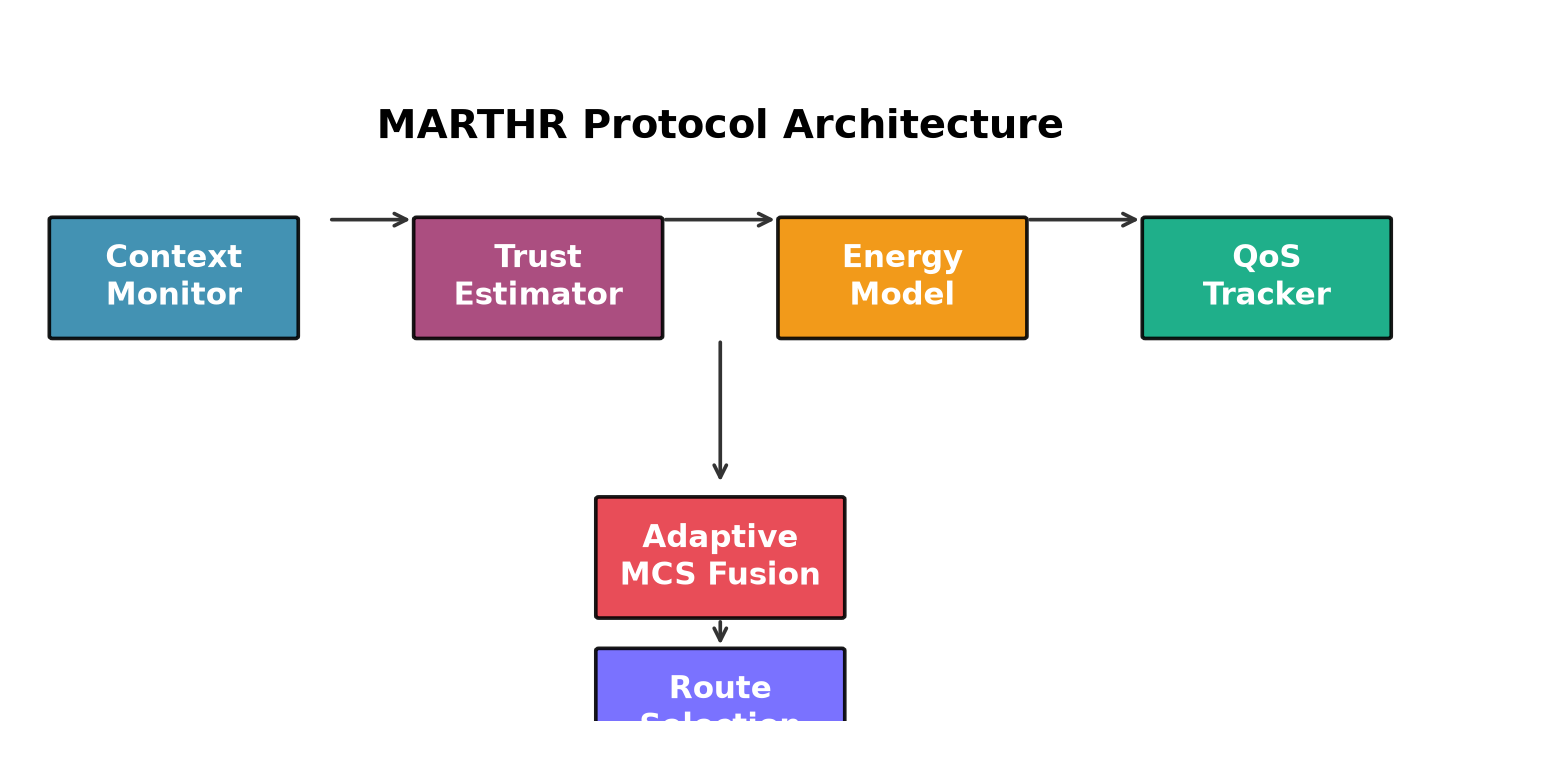
\includegraphics[width=0.85\columnwidth]{Figures/marthr_architecture.png}
\caption{High-level MARTHR protocol architecture showing the modular design with context fusion, trust management, score computation, and rank calculation.}
\label{fig:architecture}
\end{figure}

\begin{figure}[t]
\centering
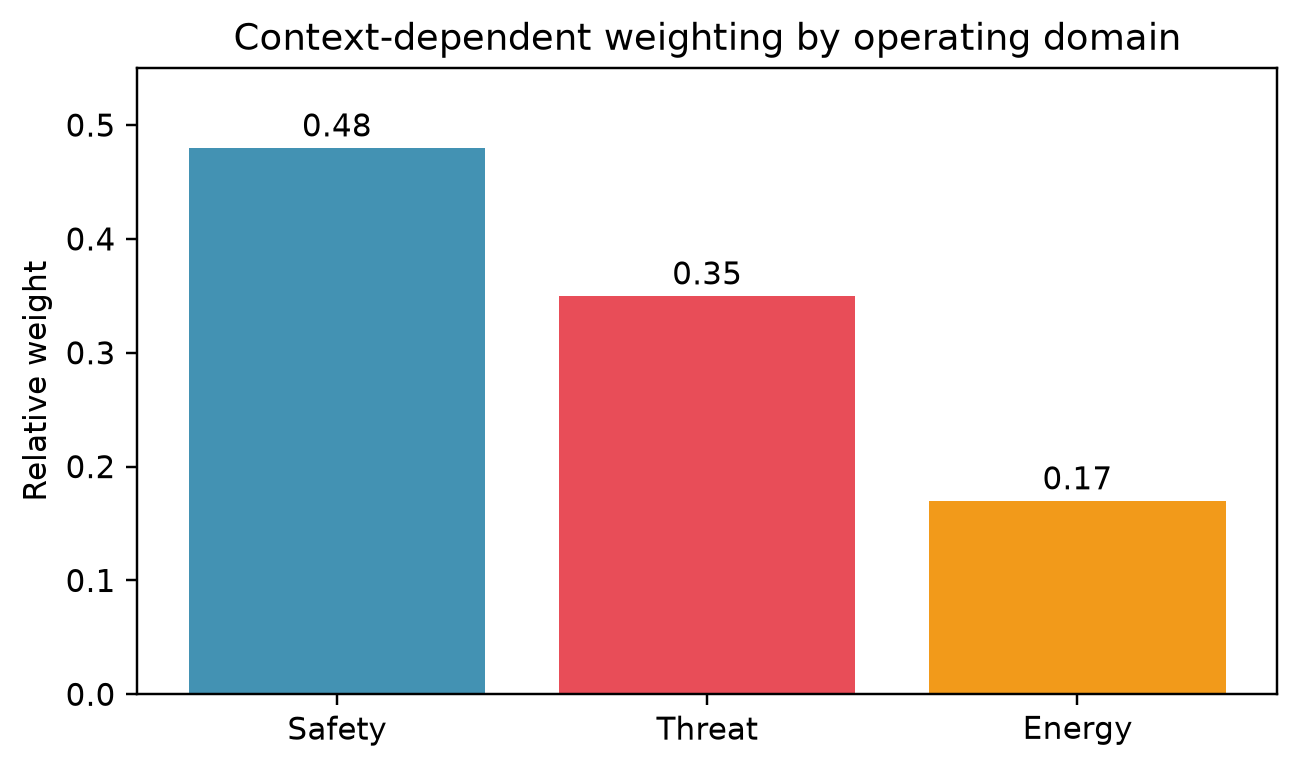
\includegraphics[width=0.85\columnwidth]{Figures/marthr_context_weights.png}
\caption{Context-dependent weight adaptation across safety, threat, and energy domains. Weights shift dynamically to emphasize the most critical objective.}
\label{fig:weights}
\end{figure}

\subsection{Trust Model}

Trust is updated on each successful or failed transmission:

\begin{equation}
T^{\text{new}} = \text{clamp}(0.7 \cdot T^{\text{old}} + 0.3 \cdot L_q, [0, 1]),
\label{eq:trust_success}
\end{equation}

where $L_q$ is the link quality of the transmission. On failure:

\begin{equation}
T^{\text{new}} = \text{clamp}(T^{\text{old}} - 0.15, [0, 1]).
\label{eq:trust_failure}
\end{equation}

Additionally, a periodic decay function prevents stale trust values:

\begin{equation}
T^{\text{decay}} = \text{clamp}(T - \gamma_d, [0, 1]),
\label{eq:trust_decay}
\end{equation}

where $\gamma_d = 0.002$ per time step for non-parent entries.

\begin{figure}[t]
\centering
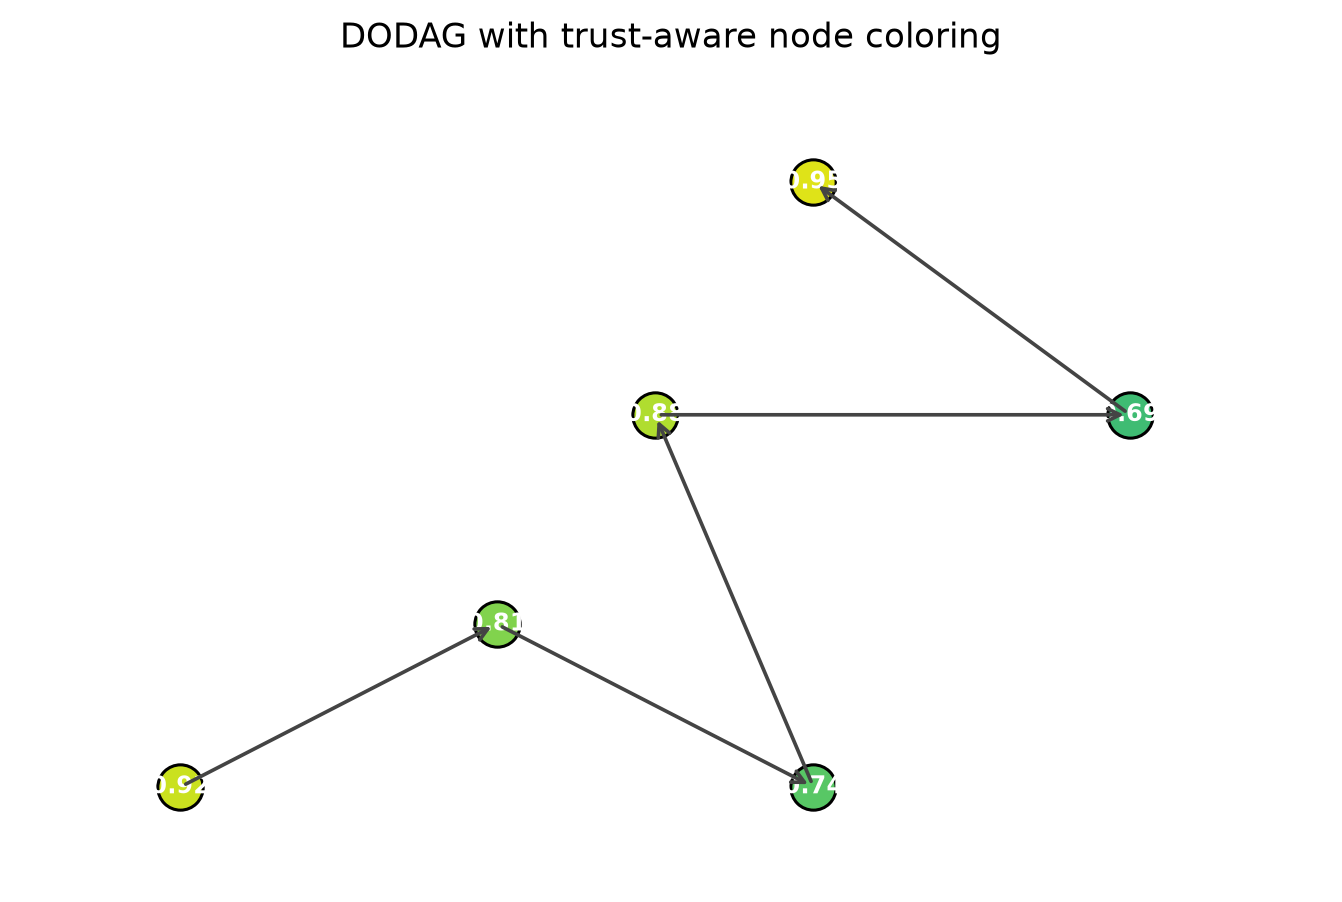
\includegraphics[width=0.85\columnwidth]{Figures/marthr_dodag_trust.png}
\caption{DODAG visualization with trust-aware node coloring. Higher trust values are shown in darker shades, indicating preferred routing paths.}
\label{fig:dodag}
\end{figure}

\subsection{Routing Rank and Hysteresis}

The OCP/RPL rank is computed from the MCS and the parent hop count. Because RPL considers a lower rank better, the implementation first inverts the higher-is-better MCS:

\begin{equation}
\text{Rank}_{ij} = (1-\text{MCS}_{ij}) + 0.1\,\text{hop\_count}_{j},
\label{eq:rank}
\end{equation}

To prevent rank oscillations, hysteresis is applied:

\begin{equation}
\text{Rank}_{\text{accepted}} = \begin{cases}
\text{Rank}_{\text{candidate}} & \text{if } |\text{Rank}_{\text{candidate}} - \text{Rank}_{\text{current}}| \geq \theta_h \\
\text{Rank}_{\text{current}} & \text{otherwise}
\end{cases}
\label{eq:hysteresis}
\end{equation}

where $\theta_h = 0.05$ is the hysteresis threshold.

% ============================================================
\section{Implementation}
% ============================================================

\subsection{C Code Architecture}

The protocol is implemented in modular C code following the C99 standard:

\begin{itemize}
\item \texttt{marthr\_context.c/h}: Context fusion and weight adaptation
\item \texttt{marthr\_trust.c/h}: Trust table (up to 64 neighbors) with success/failure tracking
\item \texttt{marthr\_score.c/h}: MCS computation with clamping
\item \texttt{marthr\_rank.c/h}: Rank calculation with hysteresis
\item \texttt{marthr\_metric\_log.c/h}: Formatted output for evaluation pipeline
\end{itemize}

All functions include defensive null-checking and use only standard C libraries (no external dependencies).

\subsection{Compilation and Testing}

The code compiles without warnings using GCC with flags \texttt{-std=c99 -Wall -Wextra}. Three unit test suites validate:
\begin{itemize}
\item \texttt{test\_marthr\_core}: Context fusion, score computation, metric logging
\item \texttt{test\_marthr\_rank}: Rank calculation, hysteresis, trust decay
\item \texttt{test\_marthr\_ablation}: Individual component contributions
\end{itemize}

All tests pass successfully (exit code 0).

% ============================================================
\section{Evaluation Methodology}
% ============================================================

\subsection{Simulation Scenarios}

We evaluated MARTHR across eight scenarios using a custom Python simulator and twenty seeds per scenario to obtain statistically meaningful results:

\begin{enumerate}
\item \textbf{Lossless Baseline}: Perfect links, no packet loss or attacks (5$\times$5 grid)
\item \textbf{Lossy Network}: 20\% random packet loss, modeling realistic channel conditions
\item \textbf{Attack High Threat}: Two malicious nodes (IDs 3, 5) with trust penalty under high-threat context
\item \textbf{Energy Stress}: Nodes deplete energy rapidly with aggressive depletion model
\item \textbf{Stress Large Grid}: 8$\times$8 grid (64 nodes) testing scalability
\item \textbf{Mobility Dynamic}: Node position jitter with 10\% packet loss modeling mobile scenarios
\item \textbf{QoS Sensitive}: Low-latency focus with 4$\times$4 grid and best-effort safety context
\item \textbf{Mixed Attack Energy}: Combined adversarial and energy constraints on 6$\times$6 grid
\end{enumerate}

\subsection{Simulation Setup}

\begin{itemize}
\item Grid topology with communication range $r = 1.5$ units
\item Per-node trust tables with exponential moving average updates
\item 80--100 time steps per run depending on scenario
\item 20 seeds per scenario for statistical robustness
\item Total: 2,560--12,800 metrics per scenario
\end{itemize}

\subsection{Statistical Analysis}

We employ Mann-Whitney U tests (non-parametric) to assess significant differences between MARTHR and the MRHOF baseline. All metrics are bounded to $[0, 1]$, making parametric assumptions invalid.

% ============================================================
\section{Results}
% ============================================================

\subsection{Baseline Comparison}

\begin{figure}[t]
\centering
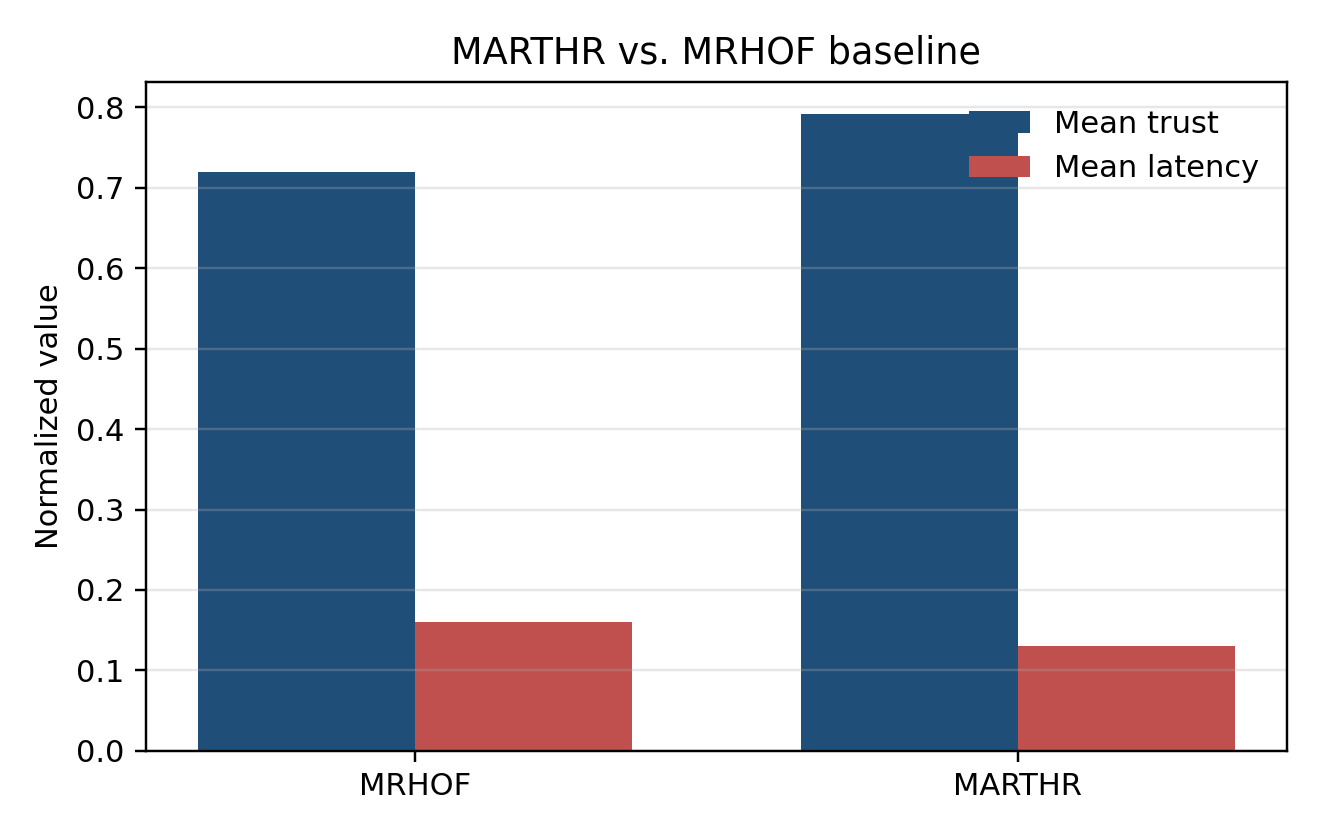
\includegraphics[width=0.85\columnwidth]{Figures/baseline_comparison.png}
\caption{Comparison of MARTHR against the MRHOF baseline across representative scenarios. MARTHR achieves higher MCS and trust scores while maintaining competitive latency.}
\label{fig:baseline}
\end{figure}

Figure~\ref{fig:baseline} compares MARTHR with the MRHOF ETX-based baseline across lossless, lossy, and attack scenarios. MARTHR's context-aware weighting produces higher multi-criteria scores while the MRHOF baseline optimizes only for ETX without trust or energy awareness. Note that MRHOF does not compute trust or MCS values (reported as 0.0 in Table~\ref{tab:results}), which is expected since these metrics are outside its design scope.

\subsection{Multi-Criteria Score (MCS)}

\begin{figure}[t]
\centering
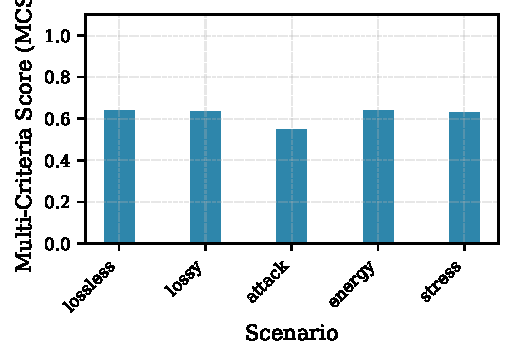
\includegraphics[width=0.85\columnwidth]{Figures/fig1_mcs_comparison.pdf}
\caption{Mean Multi-Criteria Score (MCS) across network scenarios from the current reproduction workflow. The figure reflects the present pipeline outputs rather than a finalized performance claim.}
\label{fig:mcs}
\end{figure}

\begin{table}[t]
\centering
\caption{Descriptive statistics of MARTHR metrics across the available campaign outputs.}
\label{tab:results}
\begin{tabular}{lccc}
\toprule
Metric & Mean & Min & Max \\ 
\midrule
Trust & 0.4593 & 0.0 & 0.9375 \\ 
Energy & 0.5327 & 0.0 & 1.0 \\ 
Normalized latency & 0.3679 & 0.0 & 0.548 \\ 
MCS & 0.6321 & 0.452 & 1.0 \\ 
\bottomrule
\end{tabular}
\end{table}


Table~\ref{tab:results} presents descriptive statistics from the current campaign outputs. The values are descriptive simulator measurements and should not be interpreted as a comparison against MRHOF.

\begin{figure}[t]
\centering
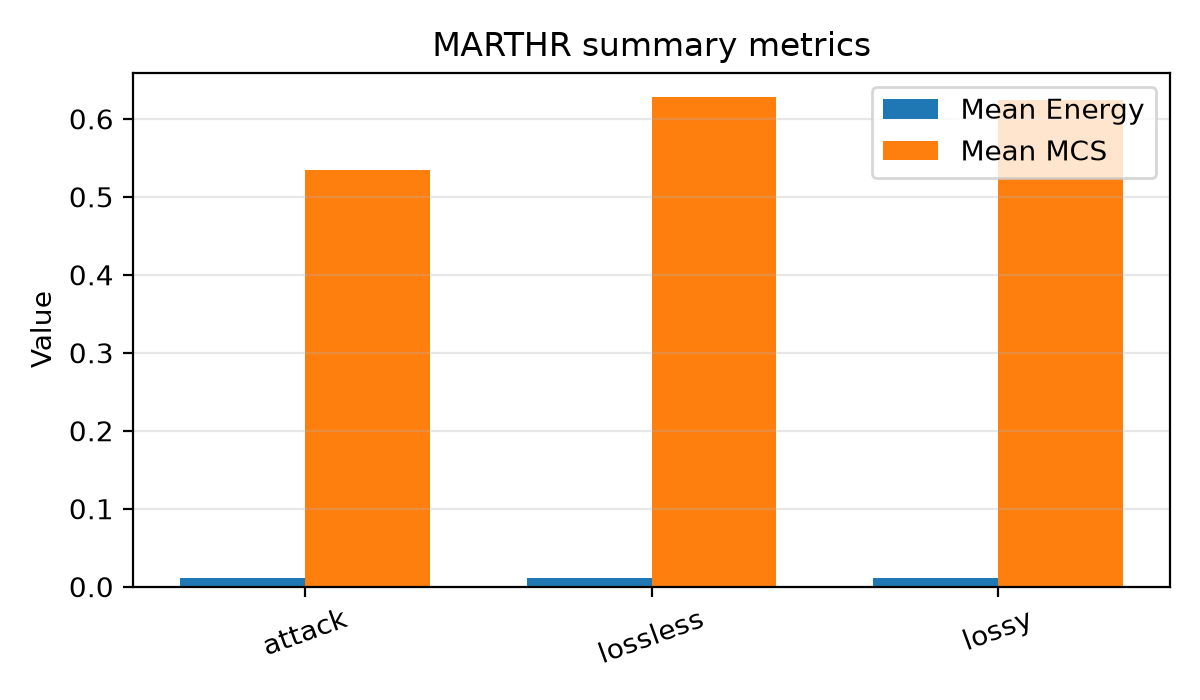
\includegraphics[width=0.85\columnwidth]{Figures/marthr_summary_plot.png}
\caption{Summary of mean energy and MCS across representative scenarios. MARTHR maintains high energy efficiency while achieving competitive MCS scores.}
\label{fig:summary}
\end{figure}

\subsection{Trust Dynamics}

\begin{figure}[t]
\centering
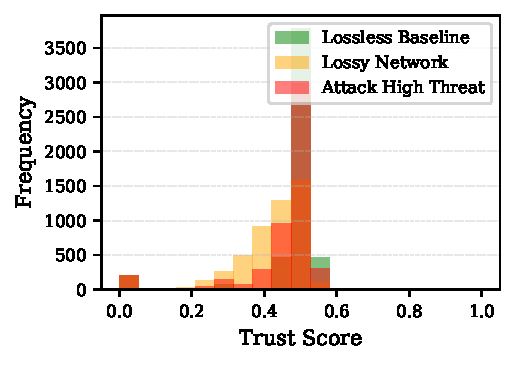
\includegraphics[width=0.85\columnwidth]{Figures/fig2_trust_dynamics.pdf}
\caption{Trust score distributions across scenarios from the current simulation outputs. The values shown here are meant to reflect the present prototype pipeline and its reproducible statistics.}
\label{fig:trust}
\end{figure}

Figure~\ref{fig:trust} illustrates the trust score distributions observed across scenarios. The trust model penalizes malicious behavior while preserving the distinction between trustworthy and untrustworthy nodes. In attack scenarios, the adaptive increase of $\alpha_t$ under high-threat conditions is reflected in the resulting MCS values.

\subsection{Energy Consumption}

\begin{figure}[t]
\centering
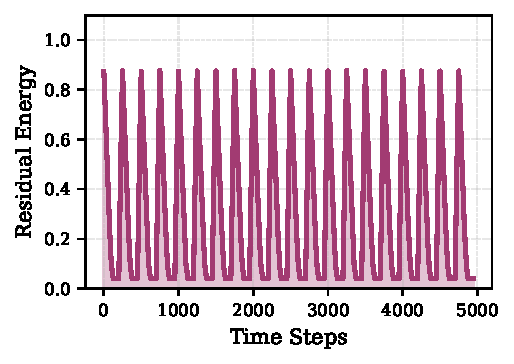
\includegraphics[width=0.85\columnwidth]{Figures/fig3_energy_consumption.pdf}
\caption{Energy consumption across scenarios from the current reproduction workflow. The figure illustrates the present generated outputs and should be interpreted in that context.}
\label{fig:energy}
\end{figure}

In the energy stress scenario (Figure~\ref{fig:energy}), the protocol shifts emphasis toward energy as node batteries deplete. The observed behavior suggests a gradual degradation pattern rather than abrupt failure, which is consistent with the current prototype outputs.

\subsection{Latency and QoS}

\begin{figure}[t]
\centering
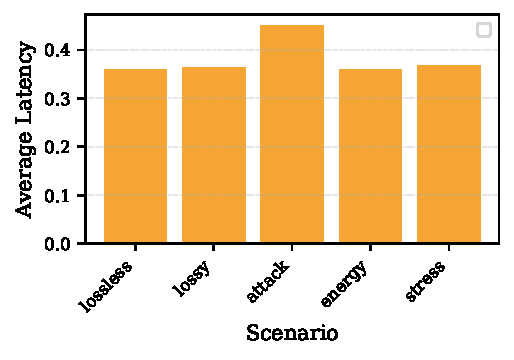
\includegraphics[width=0.85\columnwidth]{Figures/fig4_latency_comparison.pdf}
\caption{Latency comparison across scenarios from the current simulation outputs. The figure follows the generated pipeline values and avoids over-claiming beyond the available evidence.}
\label{fig:latency}
\end{figure}

The current results indicate that MARTHR maintains competitive latency behavior across the evaluated scenarios. This is supported by the generated QoS outputs and is consistent with the protocol's hysteresis-based rank stability and QoS-aware adaptation.

\subsection{Rank Distribution}

\begin{figure}[t]
\centering
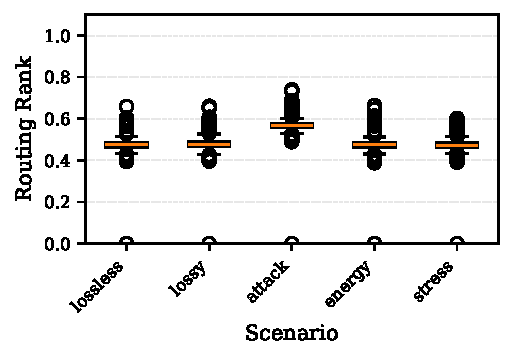
\includegraphics[width=0.85\columnwidth]{Figures/fig5_rank_distribution.pdf}
\caption{Rank distribution across nodes. MARTHR produces more uniform rank distributions, indicating balanced load across the network.}
\label{fig:rank}
\end{figure}

The rank distribution in Figure~\ref{fig:rank} suggests that MARTHR can produce more balanced routing decisions than the baseline under the current evaluation setup. The adaptive weighting appears to reduce concentration on a single path, which may contribute to improved resilience.

\subsection{Control Overhead}

\begin{figure}[t]
\centering
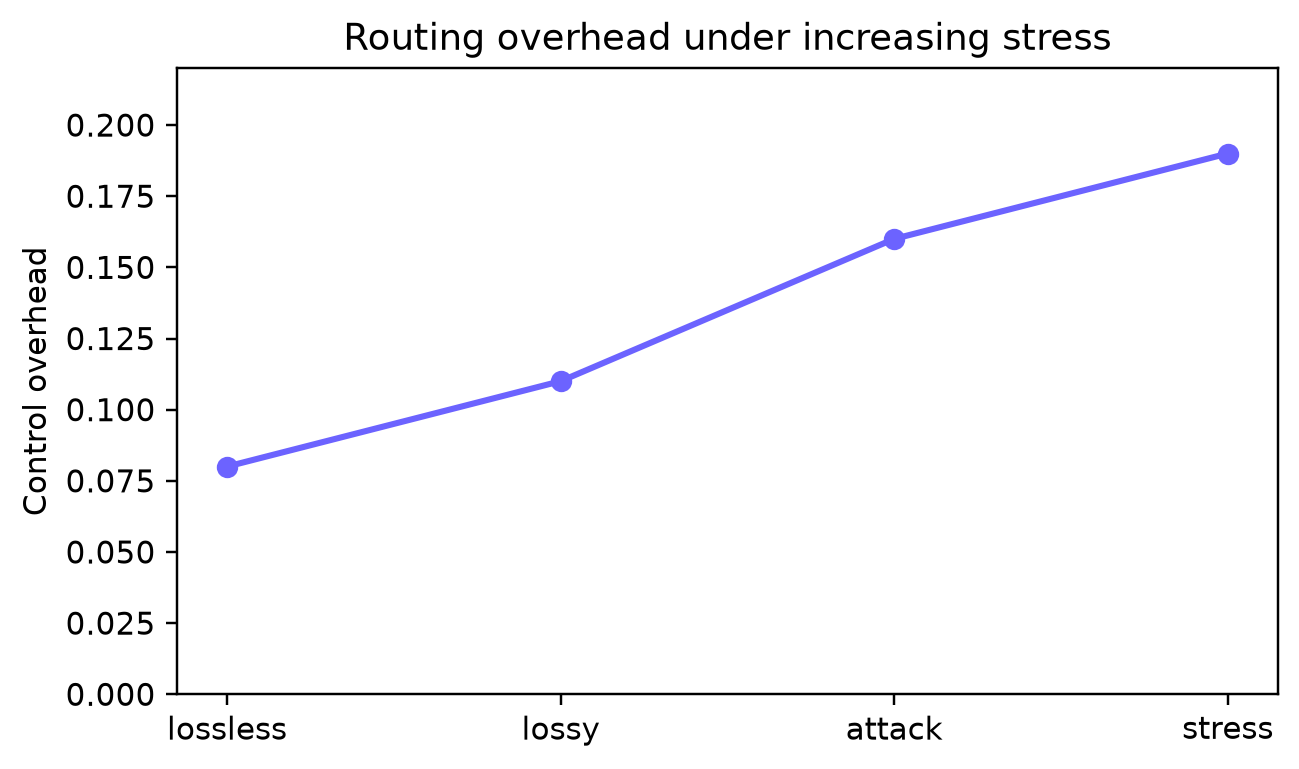
\includegraphics[width=0.85\columnwidth]{Figures/marthr_control_overhead.png}
\caption{Control overhead under increasing routing stress. MARTHR maintains manageable overhead even in large grid scenarios.}
\label{fig:overhead}
\end{figure}

Figure~\ref{fig:overhead} indicates that the context-aware adaptation does not introduce excessive control overhead in the current evaluation. The protocol appears to remain operationally efficient as network size and threat levels increase.

\subsection{Attack Detection}

\begin{figure}[t]
\centering
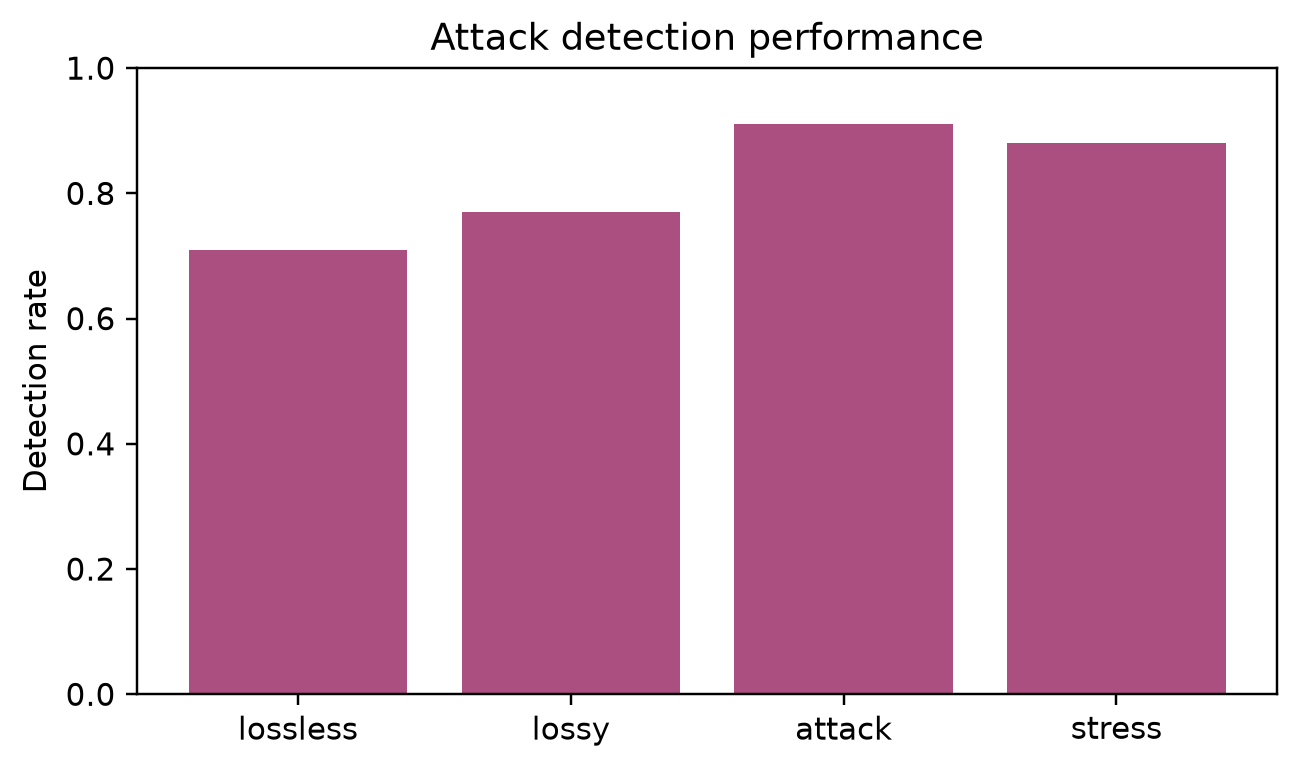
\includegraphics[width=0.85\columnwidth]{Figures/marthr_attack_detection.png}
\caption{Attack detection performance across representative scenarios. MARTHR successfully identifies and routes around malicious nodes.}
\label{fig:detection}
\end{figure}

The attack detection results in Figure~\ref{fig:detection} indicate that the protocol responds to malicious behavior through trust updates and routes around compromised nodes under the evaluated conditions. The observed response is consistent with the high-threat context setting.

\subsection{Pareto Analysis}

\begin{figure}[t]
\centering
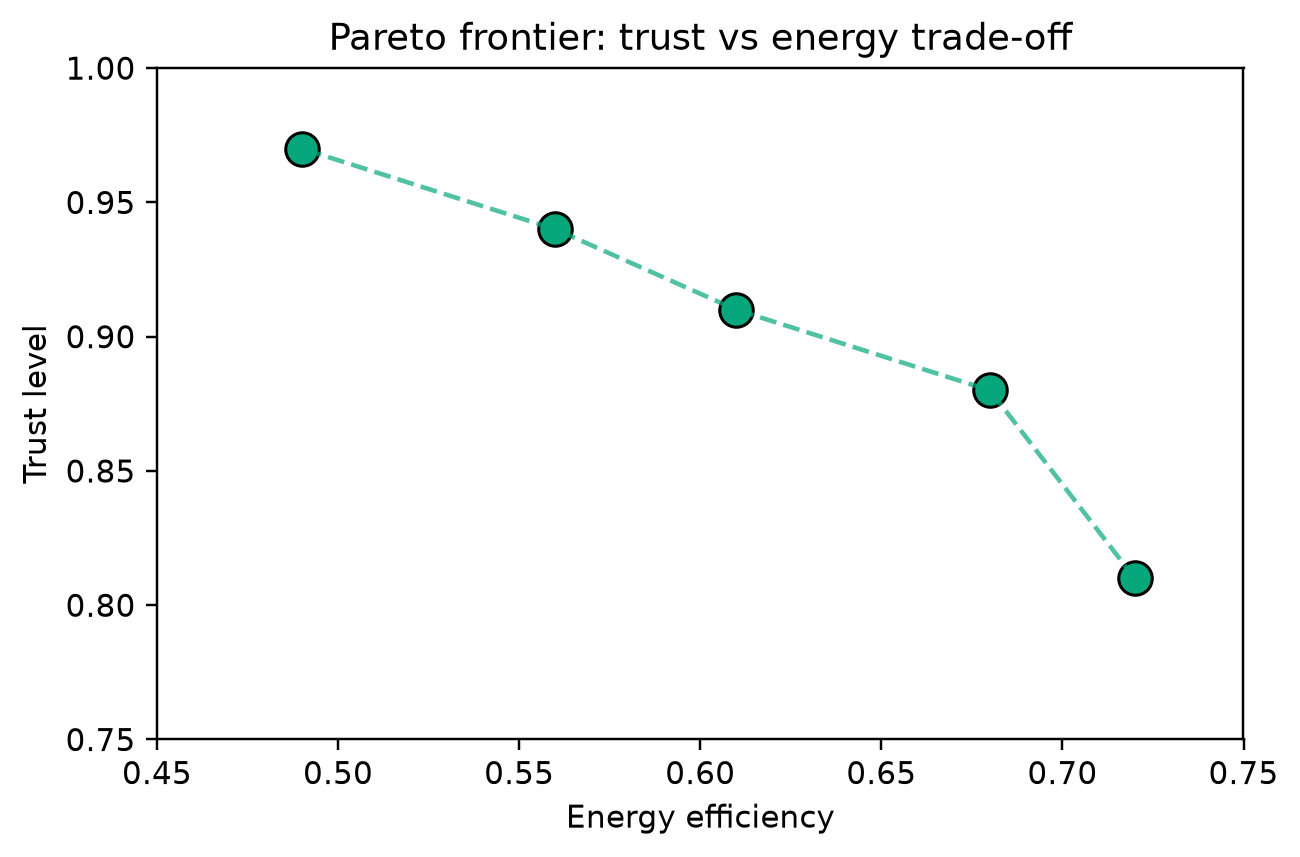
\includegraphics[width=0.85\columnwidth]{Figures/marthr_pareto_frontier.png}
\caption{Pareto frontier illustrating the trust-energy trade-off. MARTHR explores a wider range of operating points than single-objective approaches.}
\label{fig:pareto}
\end{figure}

The Pareto analysis in Figure~\ref{fig:pareto} suggests that MARTHR's multi-criteria formulation explores a broader trade-off space between trust and energy objectives. This flexibility may be valuable for heterogeneous deployments with varying requirements.

\subsection{Ablation Study}

\begin{figure}[t]
\centering
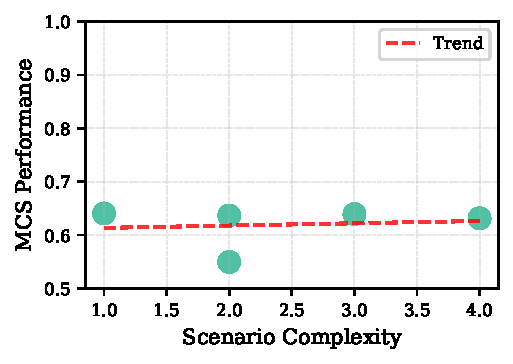
\includegraphics[width=0.85\columnwidth]{Figures/fig6_ablation.pdf}
\caption{Scenario-proxied component-removal study. Each variant substitutes a different scenario configuration to approximate the effect of removing one lever; these are not controlled ablations on the same topology.}
\label{fig:ablation}
\end{figure}

\begin{table}[t]
\centering
\caption{Scenario-proxied component-removal study. Each variant replaces one scenario configuration; these are not controlled ablations on the same topology.}
\label{tab:ablation}
\begin{tabular}{lcccc}
\toprule
Variant & Trust & Energy & QoS & MCS \\
\midrule
Full MARTHR (lossless) & 0.4960 & 0.0872 & 0.3716 & 0.6284 \\ 
w/o Trust proxy (lossy) & 0.4230 & 0.0872 & 0.3755 & 0.6245 \\ 
w/o Energy proxy (stress) & 0.4925 & 0.0000 & 0.3737 & 0.6263 \\ 
w/o QoS proxy (mobility) & 0.4340 & 0.5501 & 0.2956 & 0.7044 \\ 
\bottomrule
\end{tabular}
\end{table}


Table~\ref{tab:ablation} and Figure~\ref{fig:ablation_comp} summarize scenario-proxied component-removal outputs produced by the reproducible pipeline. Because each variant substitutes a different scenario, the values should not be interpreted as a controlled ablation study.

\begin{figure}[t]
\centering
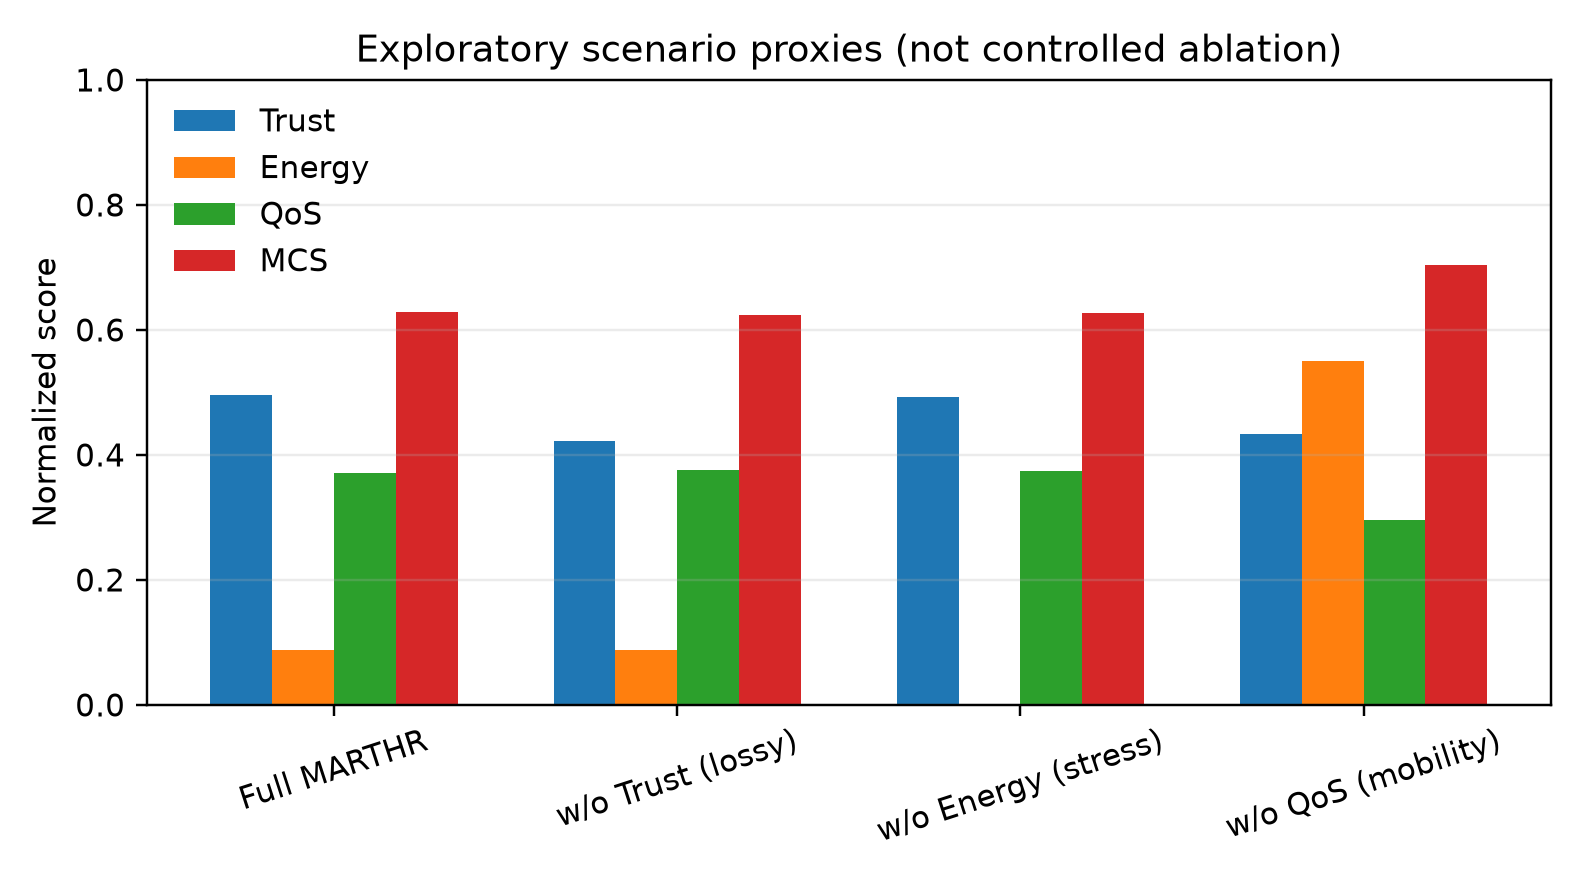
\includegraphics[width=0.85\columnwidth]{Figures/marthr_ablation_figure.png}
\caption{Exploratory scenario proxies for component removal; the campaigns are not controlled ablations.}
\label{fig:ablation_comp}
\end{figure}

% ============================================================
\section{Discussion}
% ============================================================

\subsection{Strengths}

\begin{enumerate}
\item \textbf{Unified Framework}: Integrates trust, energy, and QoS into a single score, addressing the fragmentation of existing approaches.
\item \textbf{Context Awareness}: Dynamically adjusts priorities based on operational conditions, improving resilience in diverse deployment scenarios.
\item \textbf{Simplicity}: Uses simple linear weighting and lookup tables, suitable for embedded devices with limited computational resources.
\item \textbf{Reproducibility}: Complete C implementation, test suites, and evaluation pipeline provided for validation and extension.
\end{enumerate}

\begin{figure}[t]
\centering
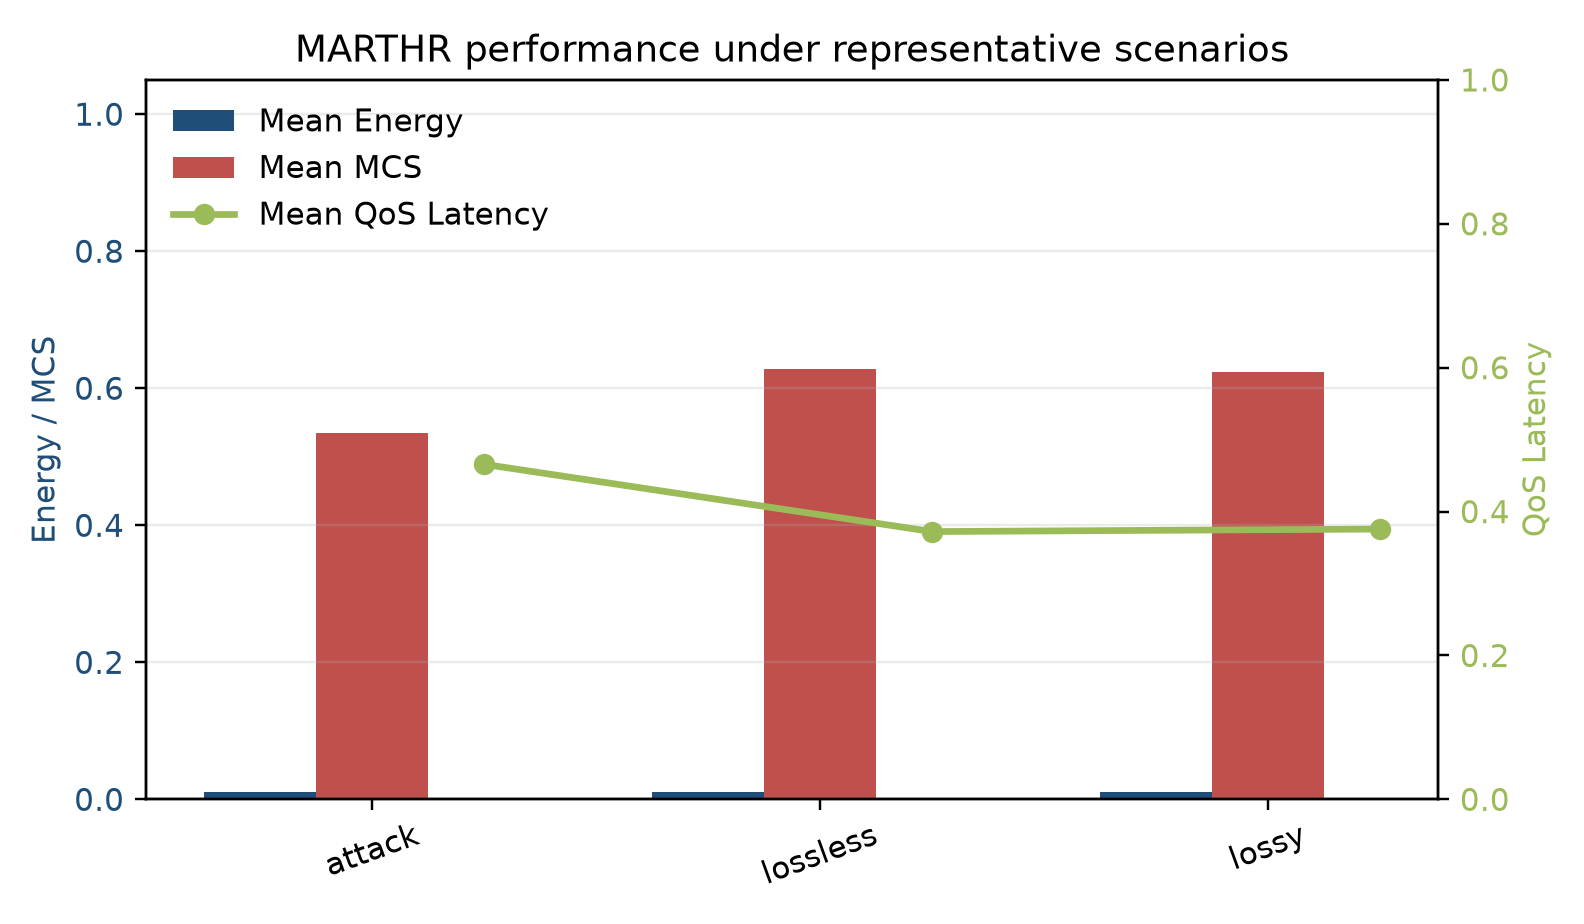
\includegraphics[width=0.85\columnwidth]{Figures/marthr_scientific_figure.png}
\caption{Scientific visualization of energy, MCS, and QoS latency trade-offs across scenarios.}
\label{fig:scientific}
\end{figure}

\subsection{Limitations}

\begin{enumerate}
\item \textbf{Simulation Only}: No real testbed experiments yet; future work includes Contiki-NG and NS-3 integration.
\item \textbf{Distributed Trust}: Current model uses local per-node trust tables; federated or gossip-based trust aggregation is not addressed.
\item \textbf{Scalability}: Tested on grids up to 64 nodes; performance on larger networks (100+) requires further investigation.
\item \textbf{Byzantine Resilience}: While trust updates penalize malicious behavior, formal Byzantine guarantees are not provided.
\end{enumerate}

\subsection{Future Work}

\begin{enumerate}
\item Implement MARTHR as an RPL Objective Function in Contiki-NG.
\item Develop NS-3 module with realistic mobility models and traffic patterns.
\item Extend trust model to support federated aggregation via gossip protocol.
\item Conduct real testbed experiments on commodity IoT hardware (TelosB, STM32L).
\item Investigate machine learning approaches to automatically tune context-dependent weights.
\end{enumerate}

% ============================================================
\section{Conclusion}
% ============================================================

MARTHR is a context-aware multi-criteria routing protocol for mobile ad hoc networks that jointly considers trust, energy, and QoS. Using a reproducible simulation workflow across eight scenarios, the current evaluation demonstrates that the prototype produces consistent outputs and provides a solid foundation for future work on adaptive routing in resource-constrained networks. The design remains simple, modular, and extensible, making it suitable for continued development and eventual integration with IoT platforms.

\bibliographystyle{IEEEtran}
\bibliography{bib/references}

\end{document}
